\section{実験装置}
\figref{fig:gamma} に実験に使用するicart-mini\cite{icart} をベースに開発したロボットを示す.
ロボットには以下に示すセンサ, PC を搭載している.
% センサとして,単眼のウェブカメラ (サンワサプライ株式会社 CMS-V43BK) を 3 つ, を 1 つ,左右のモータにそれぞれパルス付きエンコーダを搭載している.
% 制御,学習用の PC には GALLERIA GCR2070RGF-QC-G を使用している.
\begin{enumerate}
    \item [1)] ウェブカメラ (サンワサプライ株式会社 CMS-V43BK) 
    \item [2)] 2D-LiDAR (北陽電機 UTM-30LX)
    \item [3)] PC (GALLERIA GCR2070RGF-QC-G)
    \item [4)] エンコーダ
\end{enumerate}
メトリックマップに基づくルールベース制御器には,本学で ROS Navigation stack をもとに開発したorne navigation\cite{orne_nav}を使用する.

\begin{figure}[htbp]
    \centering
     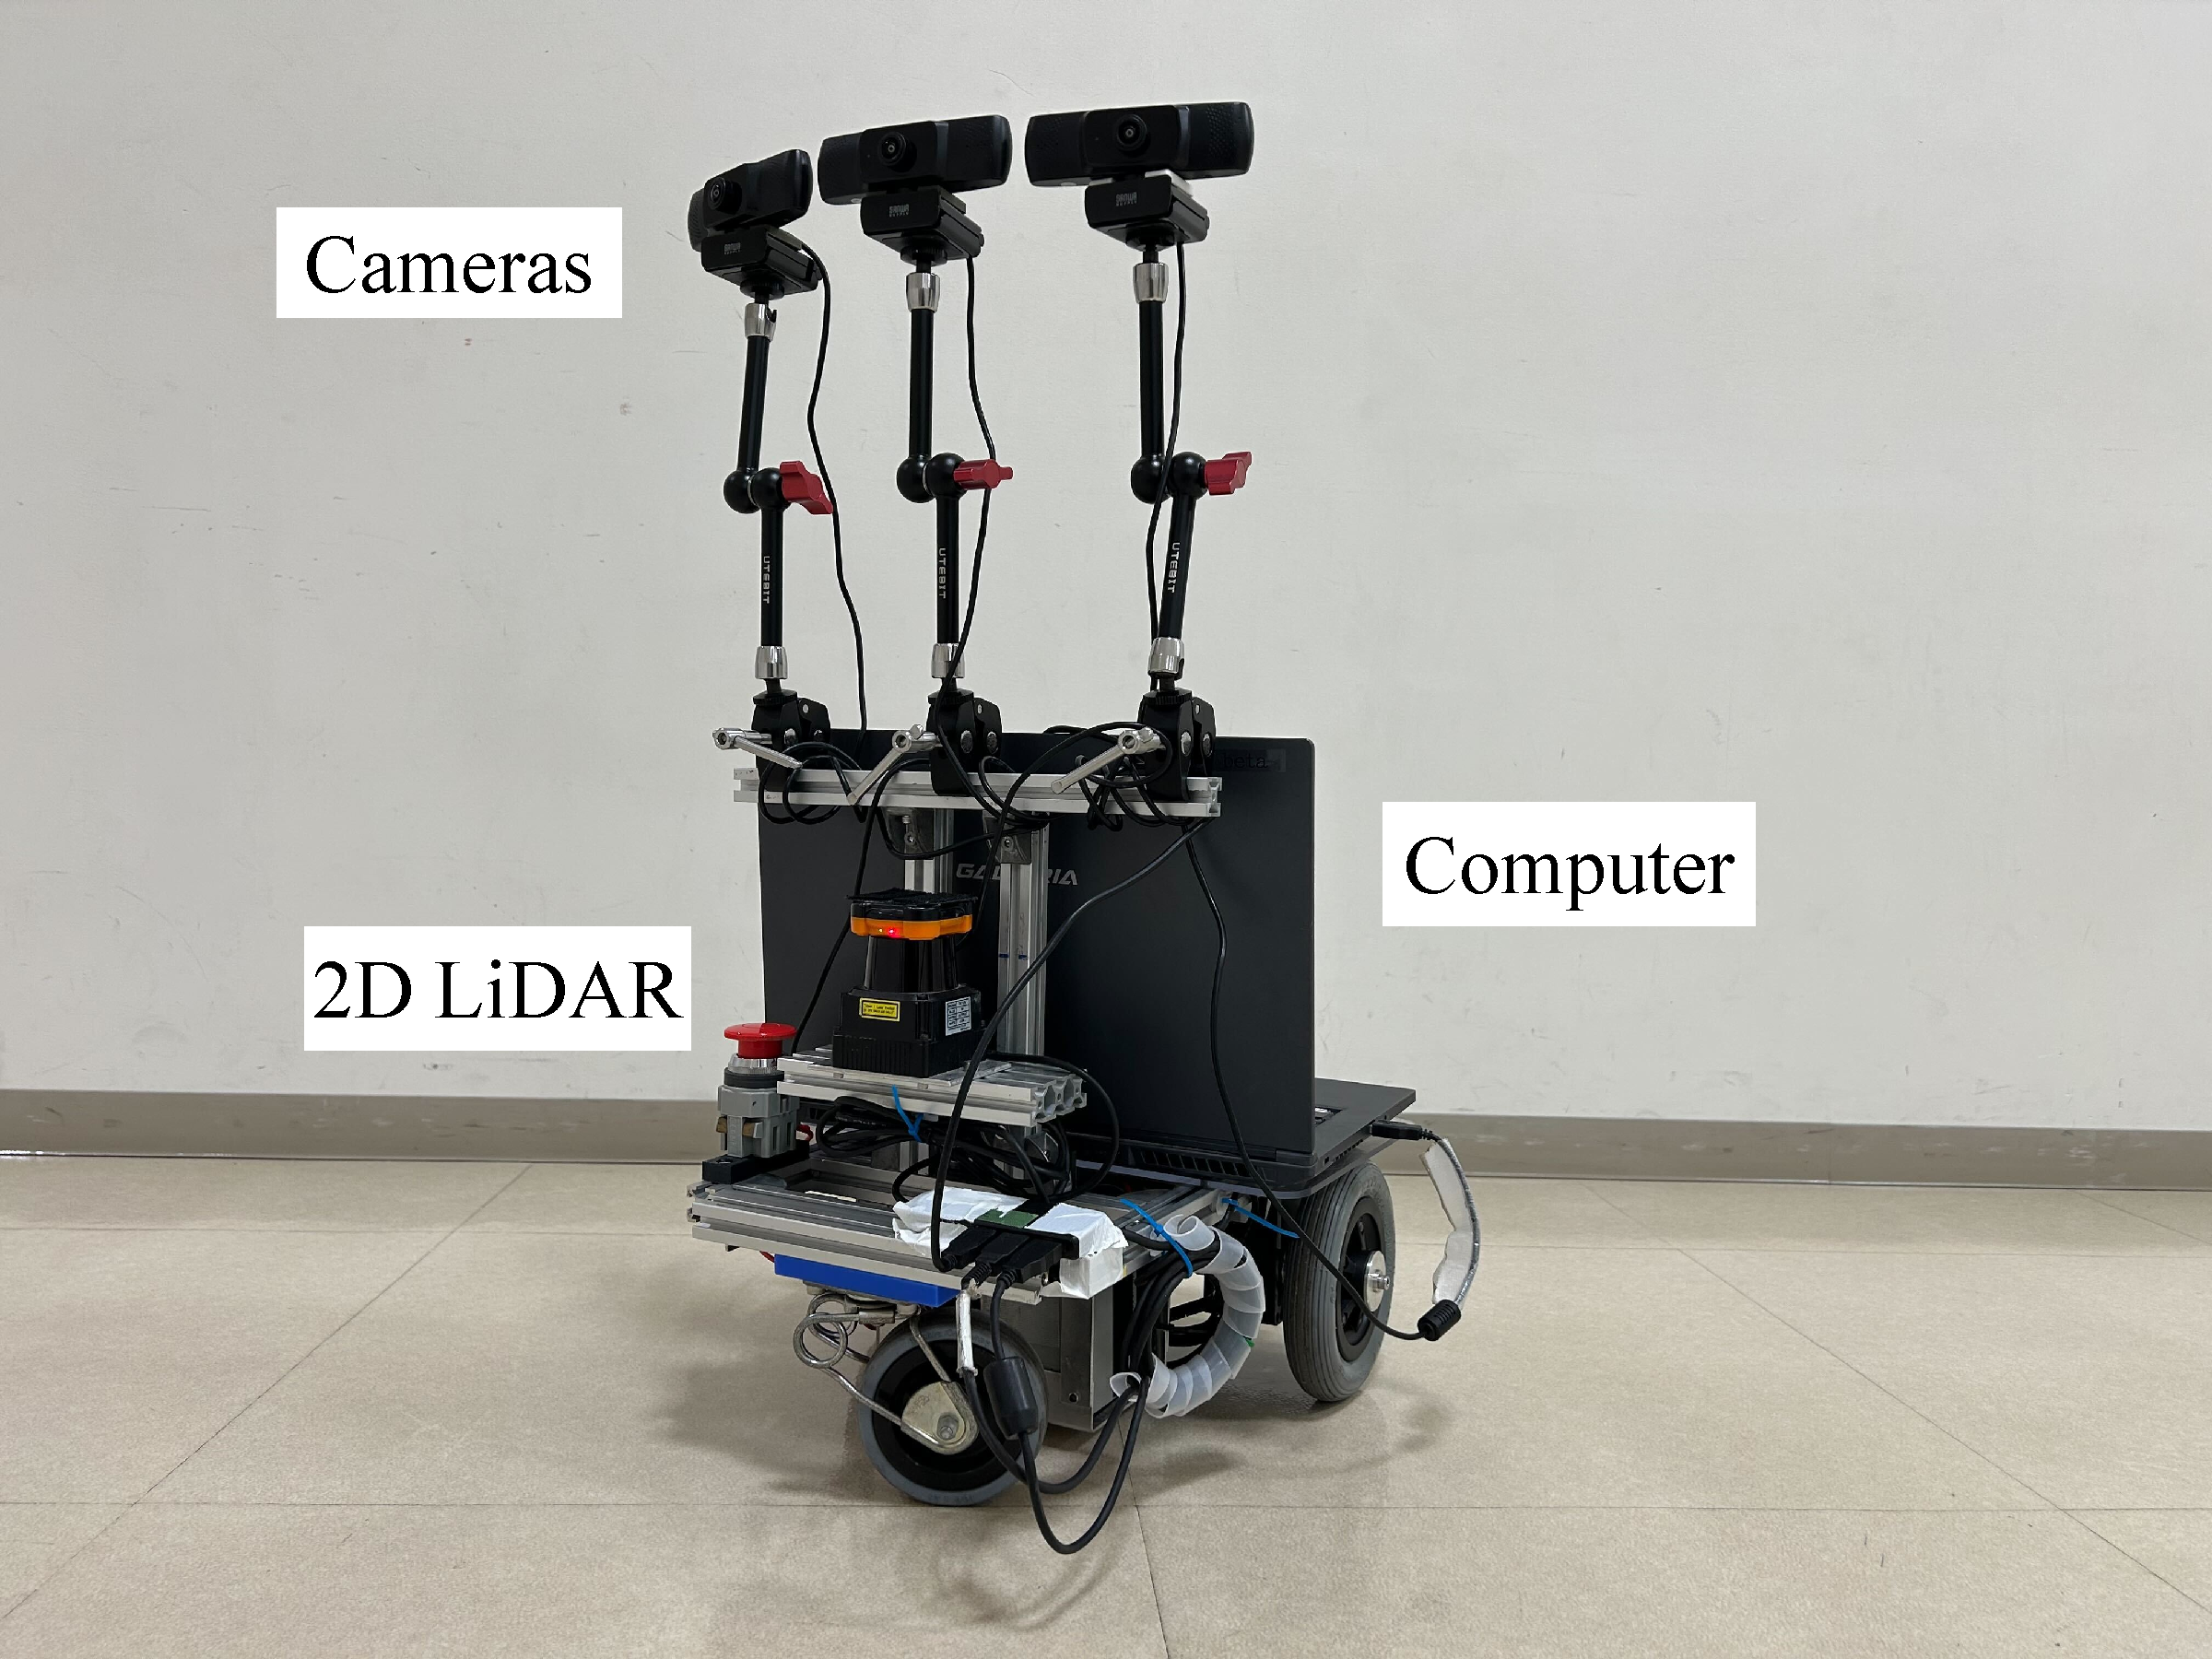
\includegraphics[width=60mm]{images/pdf/ishiguro/gamma.pdf}
     \caption{Experimental setup}
     \label{fig:gamma}
\end{figure}